% Emacs settings: -*-mode: latex; TeX-master: "manual.tex"; -*-

\chapter{Chopper-like components}

In this section, we will present rotating components such as 
chopppers, velocity selectors, {\em etc.}

\section{V\_selector: The rotating velocity selector}

The component {\bf V\_selector} models a rotating velocity
selector constructed from a number of collimator blades
arranged radially on an axis. Two identical slits 
at a 12 o'clock position allow
neutron passage at the position of the blades.
The blades are "twisted" on the axis so that a stationary 
velocity selector does not transmit any neutrons; the total
twist angle is denoted $\phi$.
By rotating the selector you allow 
transmittance of neutrons around certain velocities, given by
\begin{equation}
V_0 = \omega L / \phi ,
\end{equation}
which means that the selector has turned the twist angle
$\phi$ during the neutron flight time $L/V_0$.

Neutrons having a velocity slightly smaller or larger than $V_0$ 
will either be transmitted or absorbed depending on the exact position
of the rotator blades when the neutron enters the selector.
Assuming this position to be unknown (and assuming infinitely
thin blades), we arrive at
\begin{equation}
T = \left\{ 
 \begin{array}{ll}
 1 - (N/2\pi ) |\phi-\omega L / V| & 
        {\rm if}\,  -1 < (N/2\pi )(\phi -\omega L / V) < 1 \\
    0  &  {\rm otherwise}
 \end{array} \right.
\end{equation}
where $N$ is the number of collimator blades. 

A horisontal divergence changes the above formula because of the
angular difference between the entry and exit points of the neutron.
The resulting transmittance resembles the one above, only with 
$V$ replaced by $V_z$ and $\phi$ replaced by $(\phi +\psi )$, 
where $\psi$ is the angular difference due to
the divergence. An additional vertical divergence does not change 
this formula, but it may contribute to $\psi$.
(We have here ignored the very small non-linearity of $\psi$ along the
neutron path in case of both vertical and horisontal divergence).

Adding the effect of a finite blade thickness, $t$, reduces the transmission
by the overall amount
\begin{equation}
dT = (N t) / (2\pi r ) ,
\end{equation}
where $r$ is the distance from the rotation axis. We ignore the variation
of $r$ along the neutron path and use just the average value.

The input parameters for V\_selector are the slit dimensions,
\textit{width}, \textit{height} (in m),
the distance between apertures, $L_0$ (in m), the length of the 
collimator blades, $L_1$ (in m), the height from rotation axix to the slit
centre, $r_0$ (in m), the rotation speed $\omega$ (in rpm)
the twist angle $\phi$ (in degrees), the blade thickness $t$ (in m),
and the number of blades, $N$.

The local coordinate system is centered at the slit centre.

\section{Chopper: The disc chopper}
\label{s:chopper}

This component was contributed by Philipp Bernhardt, Lehrstuhl f\"ur
Kristallographie und Strukturphysik.

To cut a continuous neutron beam into short pulses, you can use a disc
chopper (figure~\ref{f:chopper1}). This is a fast rotating disc with the
rotating axis parallel to the neutron beam. The disk consists of neutron
absorbing materials. To form the pulses there are slits through which
the neutrons can pass.

\begin{figure}[ht]
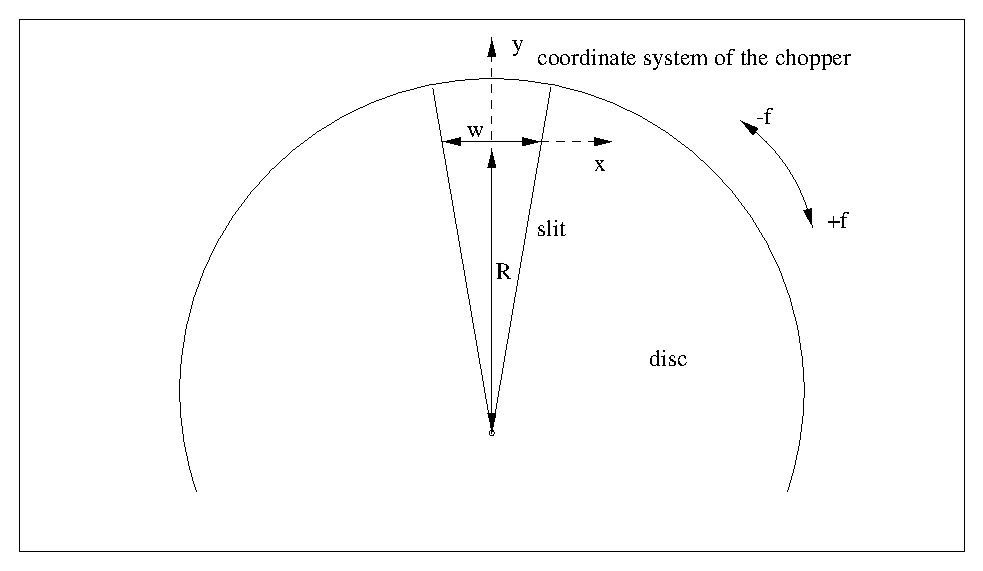
\includegraphics[width=1.0\linewidth]{figures/Chopper.eps}
\caption{disc chopper\label{f:chopper1}}
\end{figure}

This component simulates choppers with more than one slit. The slits are
symmetrically disposed on the disc. You can set the direction of
rotation, which allows to simulate double choppers. You can also define
the phase by setting the time at which one slit is positioned at the
top. The sides of the slits are pointing towards the center of the disc.
The thickness of the disc is neglected.  There is no parameter for the
height of the slits, so if you like to limit the neutrons in the
y-direction, just use a slit component in front of the chopper.

If you use a rectangular shaped beam and the beam has nearly the same
size as the slit, you will get an almost triangular shape of the
transmission curve (figure~\ref{f:chopper2}).

\begin{figure}[ht]
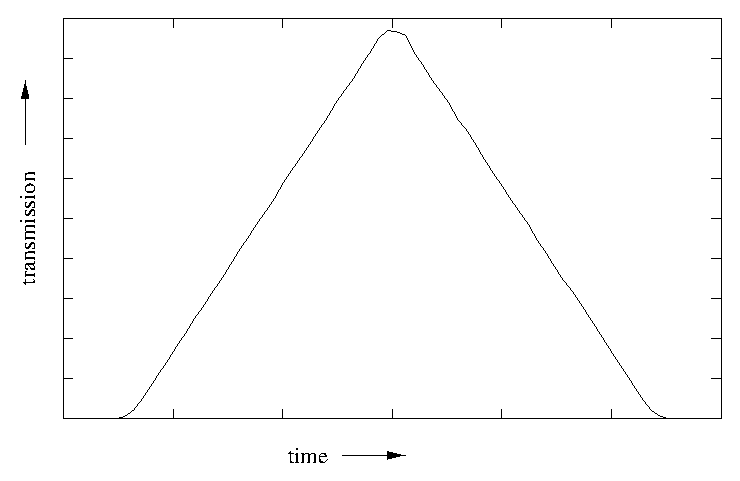
\includegraphics[width=1.0\linewidth]{figures/tracho.eps}
\caption{example transmission curve for the disc chopper\label{f:chopper2}}
\end{figure}    

The input parameters for this component are the width $w$ of the slit at
the radius $R$ of the disc, the phase \textit{pha}, the number of slits $n$ and the
angular frequency $f$. The sign of $f$ defines the direction of rotation, as
can be seen in figure~\ref{f:chopper1}.


\section{First\_chopper: The first disc chopper}
\label{s:first_chopper}

This component was contributed by Philipp Bernhardt, Lehrstuhl f\"ur
Kristallographie und Strukturphysik.

The disadvantage of the component `Chopper' is the bad statistic,
because most of the neutrons of a continuous beam are absorbed.
Furthermore TOF-instruments define the starting time of the neutrons at
the position of the first chopper and not at the source.  Therefore this
component is useful.  This `first disc chopper` has the same geometrical
and physical attributes as the normal disc chopper before.  But it
does not check if the neutron can pass the disc chopper, it instead gives
the neutron a time at which it is possible to pass. There is no
absorption in this component, all neutrons will be used.

Because the value $t$ of the incoming neutron will be overwritten, this
chopper can only be used as a first chopper.

The input parameters are, again, the width $w$ of the slit at the radius
$R$ of the disc, the phase \textit{pha} of the chopper, the number of
slits $n$ and the angular frequency $f$ (sign defines direction of
rotation). With the additional parameter $a$ you can set the number of
pulses.  This is useful if you want to investigate frame overlaps.

